\documentclass[12pt]{article}

\usepackage[a4paper,margin=2.5cm]{geometry}
\usepackage[utf8]{inputenc}
\usepackage[T1]{fontenc}
\usepackage[slovene]{babel}
\usepackage[pdfusetitle,hidelinks,unicode]{hyperref}
\usepackage{microtype}
\usepackage{graphicx}
\usepackage{float}
\usepackage{enumitem}
\usepackage{caption}
\usepackage{times}
\usepackage{amsmath}
\usepackage{amsfonts}
\usepackage{datetime}
\usepackage{csquotes}
\usepackage{listings, lstautogobble}
\usepackage{xcolor}
\usepackage[style=apa,backend=biber,maxbibnames=3,minbibnames=1,maxcitenames=2,mincitenames=1,sorting=nyt]{biblatex}
\DeclareLanguageMapping{slovene}{slovene-apa}
\addbibresource{viri.bib}

\definecolor{codebg}{RGB}{248,248,248}
\definecolor{codeframe}{RGB}{220,220,220}
\lstdefinestyle{seminarcode}{
  basicstyle=\ttfamily\small,
  backgroundcolor=\color{codebg},
  frame=single,
  rulecolor=\color{codeframe},
  captionpos=b,
  breaklines=true,
  columns=fullflexible,
  keepspaces=true,
  showstringspaces=false,
  tabsize=4
}
\lstset{style=seminarcode}
\renewcommand{\lstlistingname}{Izsek kode}

\urlstyle{rm}
\setlength{\parindent}{0pt}
\setlength{\parskip}{1ex}
\setcounter{secnumdepth}{3}
\setcounter{tocdepth}{3}
\newdateformat{MMYYYYdate}{\monthname[\THEMONTH] \THEYEAR}

\title{Nadgradnja daljinsko vodene kosilnice z ra\v{c}unalni\v{s}kim vidom in prostorskim ume\v{s}\v{c}anjem}
\author{Lin \v{C}ade\v{z}, G 4. A}

\begin{document}
\pagenumbering{arabic}

% ==============================================================
%  NASLOVNA STRAN
% ==============================================================
\begin{center}
    \thispagestyle{empty}
    \vspace{2cm}
    \\
    \textbf{Vegova ulica 4, 1000 Ljubljana}

    \vspace{\fill}
    Splo\v{s}na matura\\
    Seminarska naloga pri ra\v{c}unalni\v{s}tvu

    \Huge{\textbf{NADGRADNJA DALJINSKO VODENE KOSILNICE Z RA\v{C}UNALNI\v{S}KIM VIDOM IN PROSTORSKIM UME\v{S}\v{C}ANJEM}}

    \normalsize
    \vspace{\fill}

    Mentor: Matja\v{z} Majnik \hfill Avtor: Lin \v{C}ade\v{z}, G 4. A\\
    \null
    Ljubljana, april 2026
\end{center}

% ==============================================================
%  ZAHVALA
% ==============================================================
\newpage
\thispagestyle{empty}
\section*{Zahvala}
Zahvaljujem se mentorju Matja\v{z}u Majniku za pomo\v{c} in vodenje pri izdelavi seminarske naloge.
Posebna zahvala gre mojemu o\v{c}etu, ki mi je pomagal s finan\v{c}no podporo pri nakupu GNSS modula in
PiCama ter za potrpe\v{z}ljivost in zaupanje med testiranjem mojih novih idej na njegovem mul\v{c}erju.

% ==============================================================
%  POVZETEK
% ==============================================================
\newpage
\thispagestyle{empty}
\section*{Povzetek}
V seminarski nalogi sem nadgradil daljinsko vodeno kosilnico tako, da sem jo posku\v{s}al narediti
varnej\v{s}o in bolj pregledno za operaterja. Izhajal sem iz konkretnega problema: mul\v{c}er je te\v{z}ak,
ima ostra rezila in ga upravljam na daljavo, zato sem \v{z}elel dodati sistem, ki zazna \v{c}loveka ali
\v{z}ival in stroj samodejno ustavi. Sprva sem preizku\v{s}al enostavnej\v{s}e senzorje, vendar sem ugotovil,
da ne lo\v{c}ijo dovolj zanesljivo med ovirami in \v{z}ivimi bitji, zato sem se osredoto\v{c}il na kamero,
ra\v{c}unalni\v{s}ki vid in MobileNetSSD. Hkrati sem preveril PWM-signale daljinca, dodal spletni vmesnik
za video in polo\v{z}aj ter preizkusil DGPS z NTRIP-popravki. V nalogi sem pokazal, kaj sem v kodi
dejansko zgradil, zakaj sem izbral dolo\v{c}ene re\v{s}itve in kje so ostale omejitve.

\textbf{Klju\v{c}ne besede:} daljinsko vodena kosilnica, ra\v{c}unalni\v{s}ki vid, PWM, DGPS, NTRIP,
Raspberry~Pi

\vfill

% ==============================================================
%  KAZALO
% ==============================================================
\newpage
\tableofcontents

% ==============================================================
%  KAZALO SLIK
% ==============================================================
\newpage
\listoffigures

% ==============================================================
%  1  UVOD
% ==============================================================
\newpage
\section{Uvod}

Daljinsko vodene kosilnice se vse pogosteje uporabljajo za ko\v{s}njo te\v{z}je dostopnih terenov, kjer je
klasi\v{c}na ro\v{c}na ko\v{s}nja zahtevna ali nevarna. Opremljene so z ostrimi rezili, ki jih poganja
bencinski motor, gibanje pa omogo\v{c}ajo elektri\v{c}ni motorji in goseni\v{c}ni pogon. Zaradi tega lahko
predstavljajo resno varnostno tveganje, zlasti \v{c}e se v njihovi bli\v{z}ini znajdejo ljudje ali \v{z}ivali.
Kljub daljinskemu upravljanju ostaja odprto vpra\v{s}anje, kako zagotoviti dodatno varnost in zmanj\v{s}ati
mo\v{z}nost nesre\v{c}.

Za seminarsko nalogo sem se odlo\v{c}il na podlagi osebne izku\v{s}nje z uporabo daljinsko vodene
kosilnice. Med uporabo sem razmi\v{s}ljal, kako bi bilo mogo\v{c}e izbolj\v{s}ati varnost njenega delovanja.
Sprva sem preizku\v{s}al preproste ultrazvo\v{c}ne senzorje za zaznavanje ovir, vendar sem ugotovil, da ne
omogo\v{c}ajo zanesljivega razlikovanja med predmeti ter ljudmi in \v{z}ivalmi. Zato sem se odlo\v{c}il za
uporabo kamere in ra\v{c}unalni\v{s}kega vida, ki omogo\v{c}ata natan\v{c}nej\v{s}e zaznavanje okolice.

Namen seminarske naloge je predelava navadne daljinsko vodene kosilnice v varnej\v{s}i sistem z
zaznavanjem okolice in prostorsko umestitvijo. Cilj je razviti sistem, ki ob zaznavi \v{c}loveka ali
\v{z}ivali samodejno zaustavi kosilnico ter uporabniku omogo\v{c}a nadzor nad njenim delovanjem in
polo\v{z}ajem, pri \v{c}emer osnovno daljinsko upravljanje ostane nespremenjeno.

\begin{figure}[H]
    \centering
    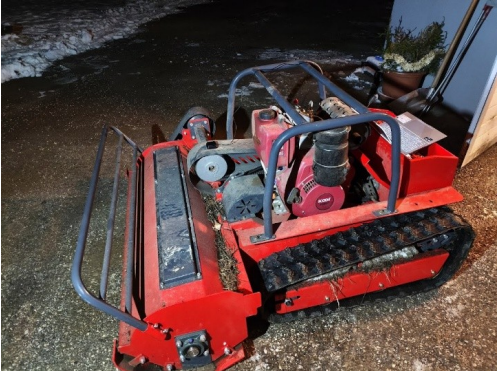
\includegraphics[width=0.82\textwidth]{slike/mulcer.png}
    \caption{Izhodi\v{s}\v{c}ni mul\v{c}er, ki sem ga uporabil za nadgradnjo.}
    \label{fig:mulcer-cover}
\end{figure}

Cilji seminarske naloge so:
\begin{itemize}[leftmargin=1.6em]
  \item analizirati delovanje daljinskega upravljanja kosilnice in PWM-signalov,
  \item izbrati primeren sistem za zaznavanje ljudi in \v{z}ivali z uporabo kamere,
  \item razviti varnostni mehanizem za samodejno zaustavitev kosilnice,
  \item preizkusiti prostorsko umestitev kosilnice z uporabo diferencialnega GPS,
  \item izdelati osnovni spletni vmesnik za spremljanje delovanja sistema.
\end{itemize}

Hipoteza seminarske naloge je, da je z uporabo ra\v{c}unalni\v{s}kega vida mogo\v{c}e zanesljivo zaznati
ljudi in \v{z}ivali v okolici kosilnice ter s tem prepre\v{c}iti morebitne po\v{s}kodbe.

Raziskovalne metode so temeljile na eksperimentalnem delu, meritvah signalov, prakti\v{c}nih preizkusih
delovanja sistema in analizi rezultatov testiranj na terenu.

% ==============================================================
%  2  JEDRO
% ==============================================================
\section{Jedro}

\subsection{Daljinsko vodene kosilnice in varnostni izzivi}

Daljinsko vodene kosilnice so posebna vrsta delovnih strojev, namenjenih ko\v{s}nji trave in
vzdr\v{z}evanju povr\v{s}in, kjer bi bila klasi\v{c}na ko\v{s}nja z ro\v{c}no ali traktorsko kosilnico neugodna
oziroma celo nevarna, na primer na strmih pobo\v{c}jih, v trnju ali na drugih te\v{z}je dostopnih terenih.
Upravljanje poteka z brez\v{z}i\v{c}nim daljinskim upravljalnikom, kar omogo\v{c}a, da se operater nahaja na
varni razdalji od stroja. Tak\v{s}ne kosilnice se pogosto uporabljajo na strmih pobo\v{c}jih, ob cestah,
na bre\v{z}inah in drugih zahtevnih terenih, kjer obstaja ve\v{c}ja nevarnost zdrsa ali izgube nadzora nad
strojem.

Delovanje daljinsko vodenih kosilnic temelji na kombinaciji mehanskega in elektri\v{c}nega pogona.
Rezalni sistem obi\v{c}ajno poganja bencinski motor, ki omogo\v{c}a visoko mo\v{c} in u\v{c}inkovito ko\v{s}njo,
medtem ko za premikanje in krmiljenje pogosto skrbijo elektromotorji, povezani z goseni\v{c}nim ali
kolesnim pogonom. Ukazi z daljinskega upravljalnika se do kosilnice prena\v{s}ajo v obliki
PWM-signalov, ki dolo\v{c}ajo smer, hitrost gibanja ter druge funkcije stroja.

Kljub temu pa tak\v{s}ne kosilnice predstavljajo resne varnostne izzive. Najve\v{c}jo nevarnost
predstavljajo hitro vrte\v{c}a se rezila, ki lahko ob stiku povzro\v{c}ijo hude telesne po\v{s}kodbe. Dodatno
tveganje izhaja iz samega gibanja stroja, saj lahko na neravnem ali strmem terenu pride do
nenadnega zdrsa, prevra\v{c}anja ali nenadzorovanega premika. Posebej nevarne so situacije, ko se v
neposredni bli\v{z}ini kosilnice znajdejo ljudje ali \v{z}ivali, saj operater kljub daljinskemu upravljanju
morda ne zazna pravo\v{c}asno vseh ovir v okolici.

Zaradi teh nevarnosti se v praksi uporabljajo razli\v{c}ni varnostni pristopi. Med najpogostej\v{s}imi so
mehanski za\v{s}\v{c}itni pokrovi rezil, sistemi za takoj\v{s}nje izklapljanje rezil ob dolo\v{c}enih pogojih ter
osnovni senzorji, ki zaznajo nagib ali dvig stroja. V strokovni literaturi je poudarjeno, da
daljinsko upravljanje samo po sebi \v{s}e ne zagotavlja popolne varnosti, temve\v{c} je potrebno
varnostne mehanizme obravnavati kot sestavni del celotnega sistema \parencite{polc2013}.

V svojem projektu sem za to uporabil \texttt{rpicam-detect}, ki temelji na modelu MobileNet~SSD
in omogo\v{c}a prepoznavanje ljudi, ma\v{c}k, avtomobilov in drugih objektov
\parencite{raspi_camera_software}.

\subsection{Elektronsko zaznavanje okolice pri delovnih strojih}

Pri delovanju avtonomnih ali daljinsko vodenih strojev je zanesljivo zaznavanje okolice klju\v{c}no za
varno navigacijo in izogibanje oviram. Razli\v{c}ne vrste senzorjev omogo\v{c}ajo strojem, da zaznajo
predmete, ovire in spremembe v okolju ter se nanje ustrezno odzovejo.

\textbf{Ultrazvo\v{c}ni senzorji} delujejo tako, da oddajajo zvo\v{c}ne valove nad \v{c}love\v{s}kim slu\v{s}nim
obmo\v{c}jem in merijo \v{c}as, ki ga potrebuje signal, da se odbije od ovire in se vrne do sprejemnika.
Na podlagi tega izra\v{c}unajo razdaljo do ovire, kar omogo\v{c}a sprotno zaznavanje prisotnosti predmetov
v bli\v{z}ini. Tak\v{s}ni senzorji so cenovno ugodni, vendar ne omogo\v{c}ajo zanesljivega razlikovanja med
razli\v{c}nimi vrstami objektov.

\textbf{Infrarde\v{c}i senzorji} zaznavajo spremembe v infrarde\v{c}em svetlobnem spektru. Uporabni so za
zaznavanje premikanja in prisotnosti predmetov v bli\v{z}ini, vendar imajo kraj\v{s}i doseg od ultrazvo\v{c}nih
sistemov in so bolj ob\v{c}utljivi na svetlobne razmere ter temperaturne spremembe. Za poletno ko\v{s}njo
tak\v{s}ni senzorji niso najbolj primerni, saj so lahko zunanje temperature zelo visoke, v\v{c}asih celo
primerljive ali vi\v{s}je od temperature \v{c}love\v{s}kega telesa. Zaradi tega je razlikovanje med \v{z}ivim
bitjem in segreto okolico manj zanesljivo.

\textbf{Sistem zaznavanja s pomo\v{c}jo kamer} zajema vizualne podatke, ki jih procesira programska
oprema za identificiranje, kategorizacijo ter dolo\v{c}anje polo\v{z}aja objektov v okolici stroja.
Kamere omogo\v{c}ajo bistveno bogatej\v{s}e informacije o okolju kot enostavni senzorji, saj omogo\v{c}ajo
detekcijo, sledenje in razlikovanje med razli\v{c}nimi vrstami ovir. Tak\v{s}ne zmogljivosti so klju\v{c}ne
pri nalogah, kjer je treba razlikovati med premi\v{c}nimi in nepremi\v{c}nimi predmeti ter zaznavati ljudi
ali \v{z}ivali.

\subsection{Pregled tehnologij}

Pred za\v{c}etkom razvoja sem moral izbrati ustrezne tehnologije za vsak podsistem. Iskal sem
majhen in var\v{c}en ra\v{c}unalnik, ki bi ga lahko enostavno vgradil v omejen prostor v \v{s}katli z
elektroniko v kosilnici. Prav tako sem moral dose\v{c}i, da je programska oprema dovolj hitra pri
zaznavanju ovir. Zastavil sem si cilj, da od zaznave ovire do zaustavitve kosilnice ne sme prete\v{c}i
ve\v{c} kot 700\,ms. Obenem sem si \v{z}elel tudi skoraj trenutni prenos slike s kosilnice na spletni
vmesnik. Tega cilja mi sicer ni uspelo dose\v{c}i popolnoma, vendar sem zakasnitev zmanj\v{s}al na
pribli\v{z}no 1 do 1{,}1\,s, kar je bilo za prakti\v{c}no uporabo \v{s}e sprejemljivo.

\begin{figure}[H]
    \centering
    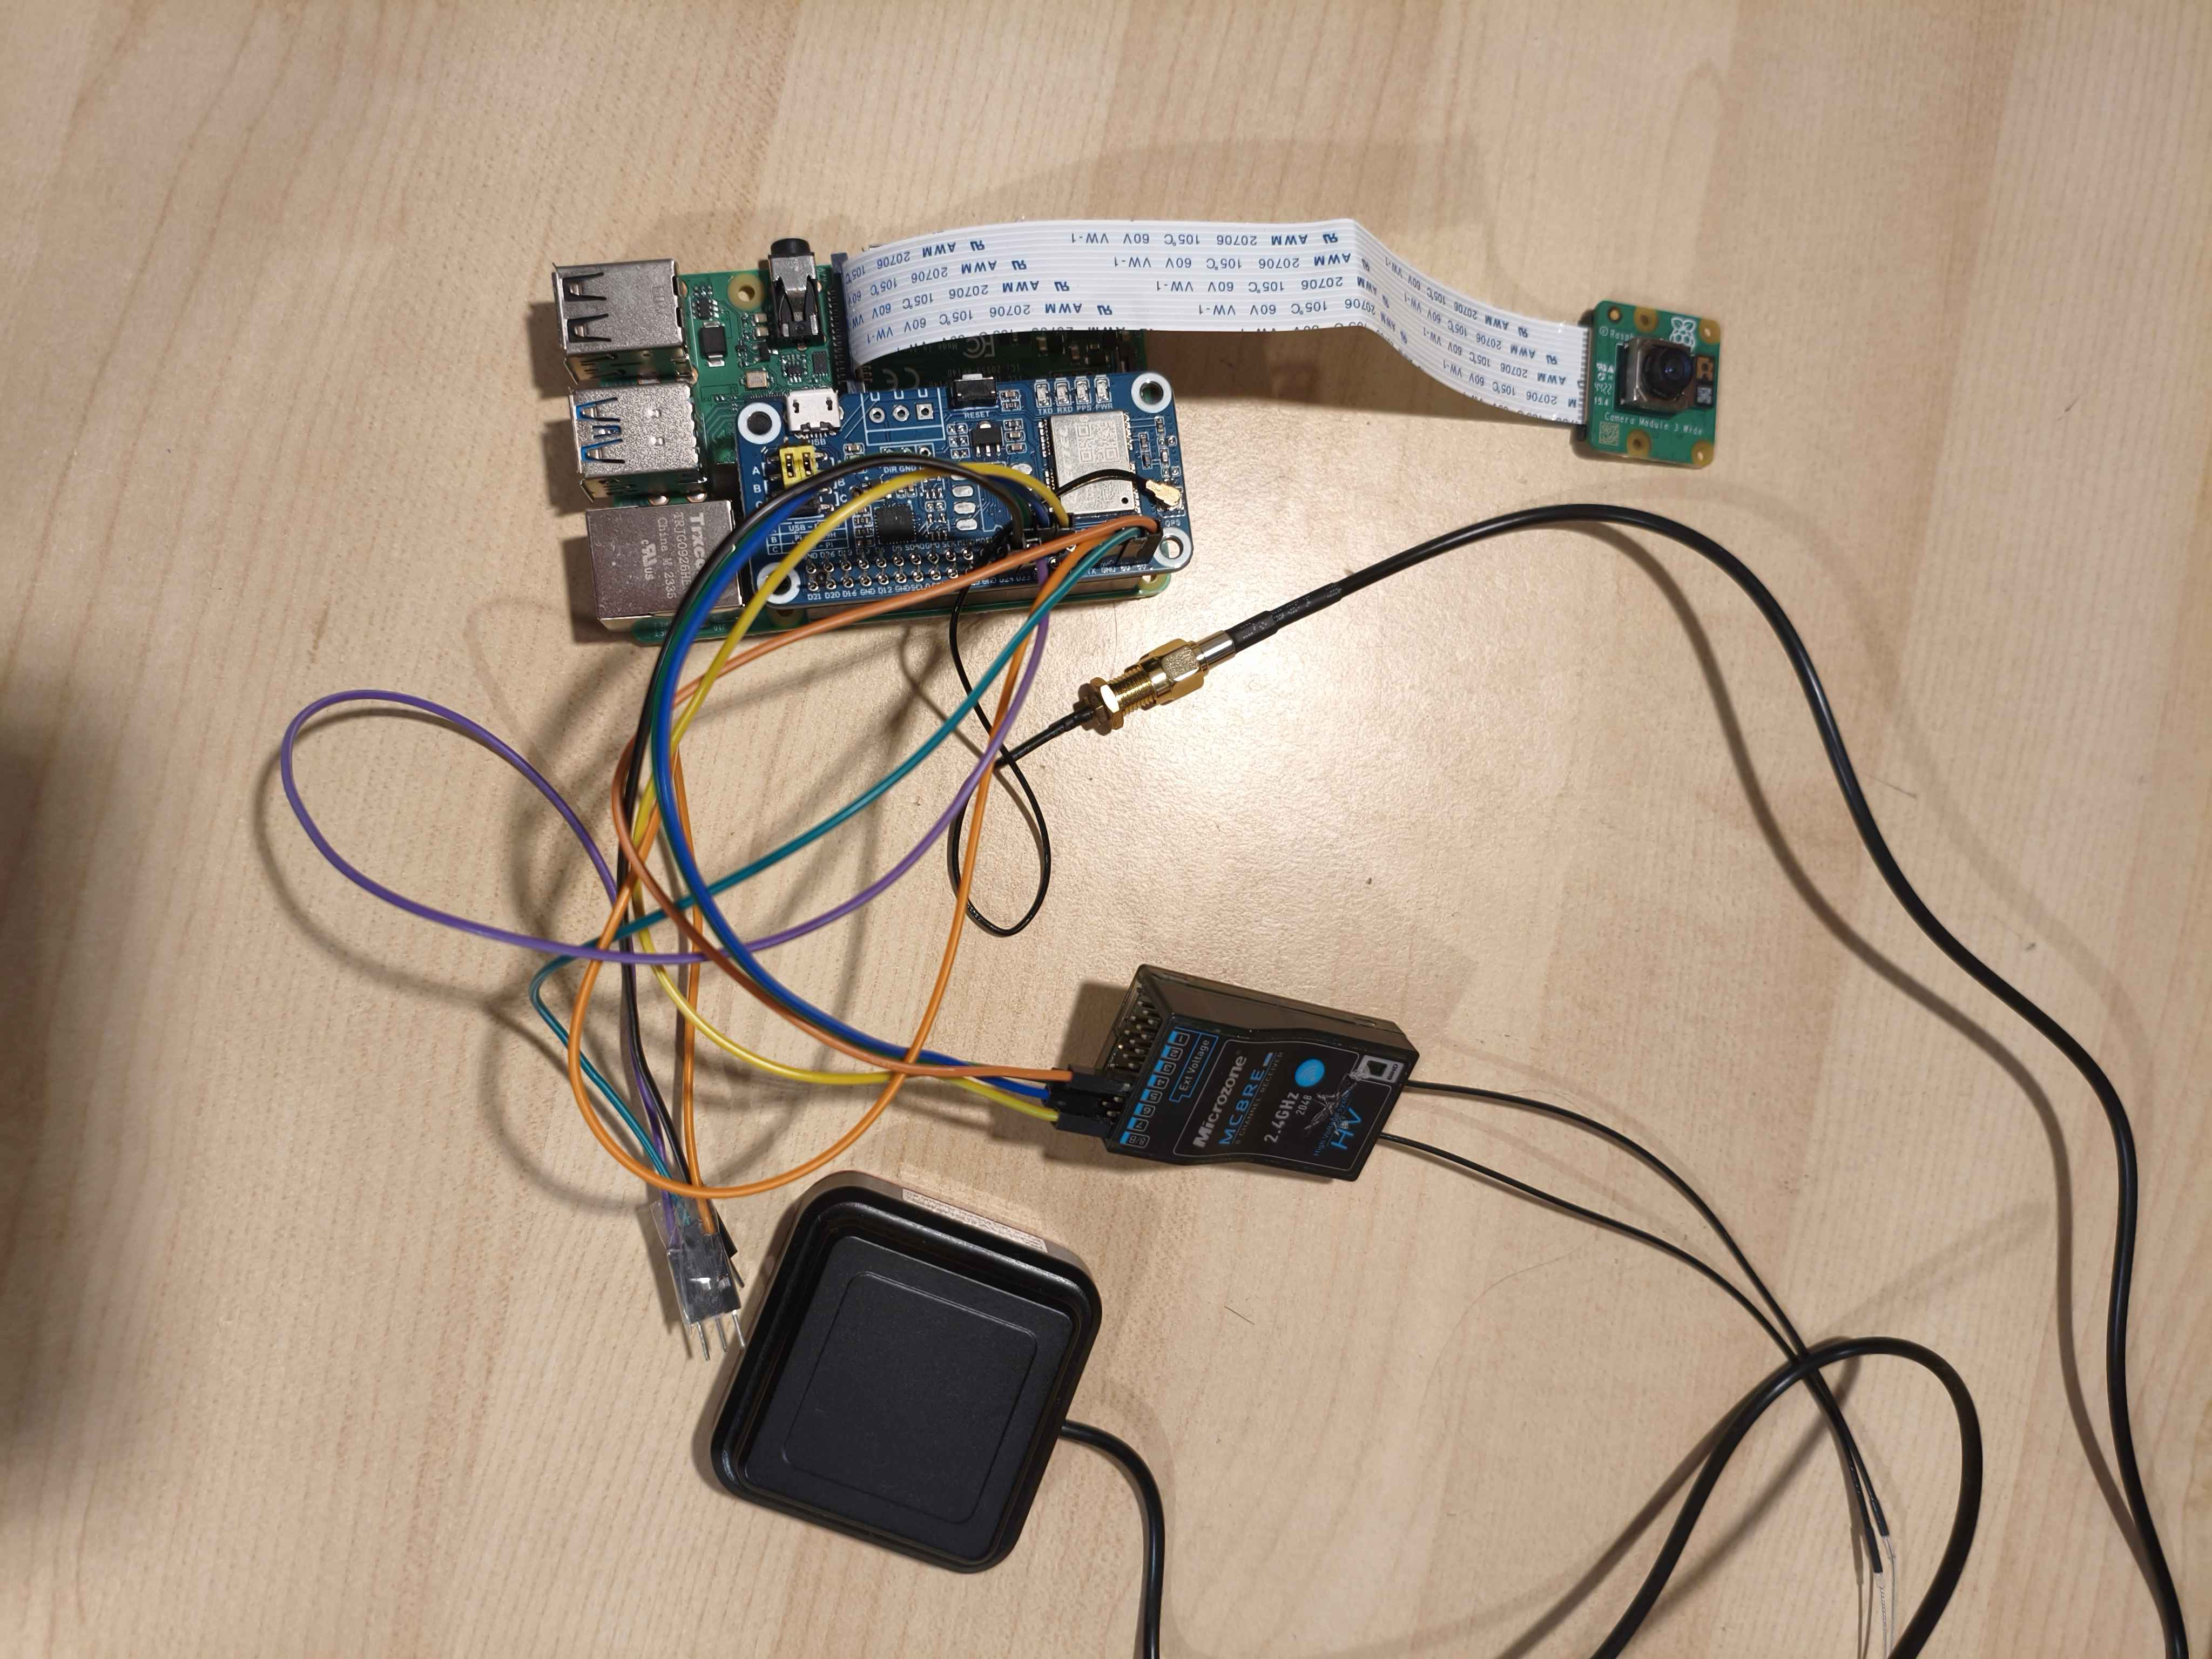
\includegraphics[width=0.78\textwidth]{slike/moduli_sistema.jpg}
    \caption{Vsi moduli sistema, povezani skupaj: GPS \v{s}\v{c}it, RC sprejemnik, PiCam, Raspberry~Pi in GPS antena.}
    \label{fig:moduli-skupaj}
\end{figure}

\subsubsection{Raspberry Pi 4B}

Raspberry~Pi~4B je ra\v{c}unalnik z vgrajenimi GPIO-priklju\v{c}ki, CSI-vmesnikom za kamero, modulom
Wi-Fi in operacijskim sistemom Linux (Raspberry~Pi~OS). Izbral sem ga, ker je dovolj majhen, da sem
ga lahko namestil neposredno v kosilnico. Za njegovo delovanje zadostuje napetost 5\,V, zato sem ga
lahko priklju\v{c}il neposredno na elektroniko kosilnice, kjer sta bili na voljo napetosti 5\,V in 12\,V.
Pomembna prednost je bila tudi dobra podpora za Python, OpenCV in delo s kamero, kar mi je bistveno
olaj\v{s}alo razvoj sistema.

\begin{figure}[H]
    \centering
    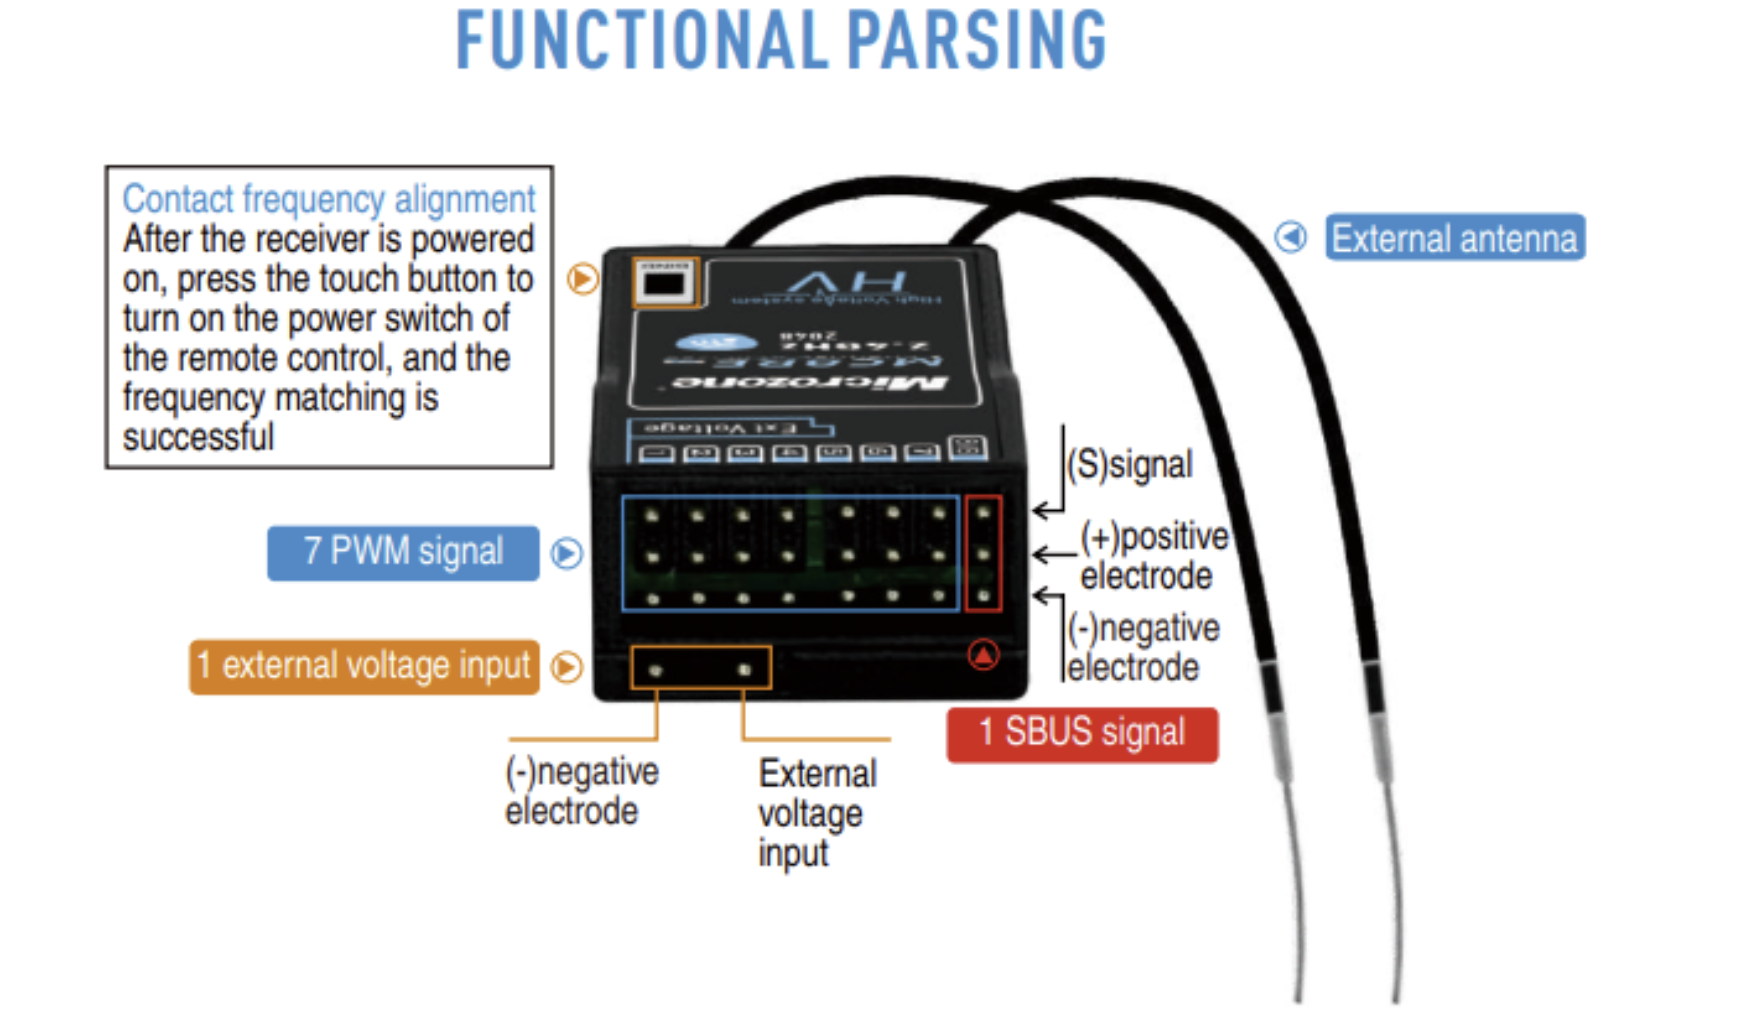
\includegraphics[width=0.72\textwidth]{slike/shema_sprejemnika.png}
    \caption{Shema priklju\v{c}kov sprejemnika iz dokumentacije, ki sem jo uporabil pri na\v{c}rtovanju GPIO-vezave.}
    \label{fig:receiver-pinout}
\end{figure}

\begin{figure}[H]
    \centering
    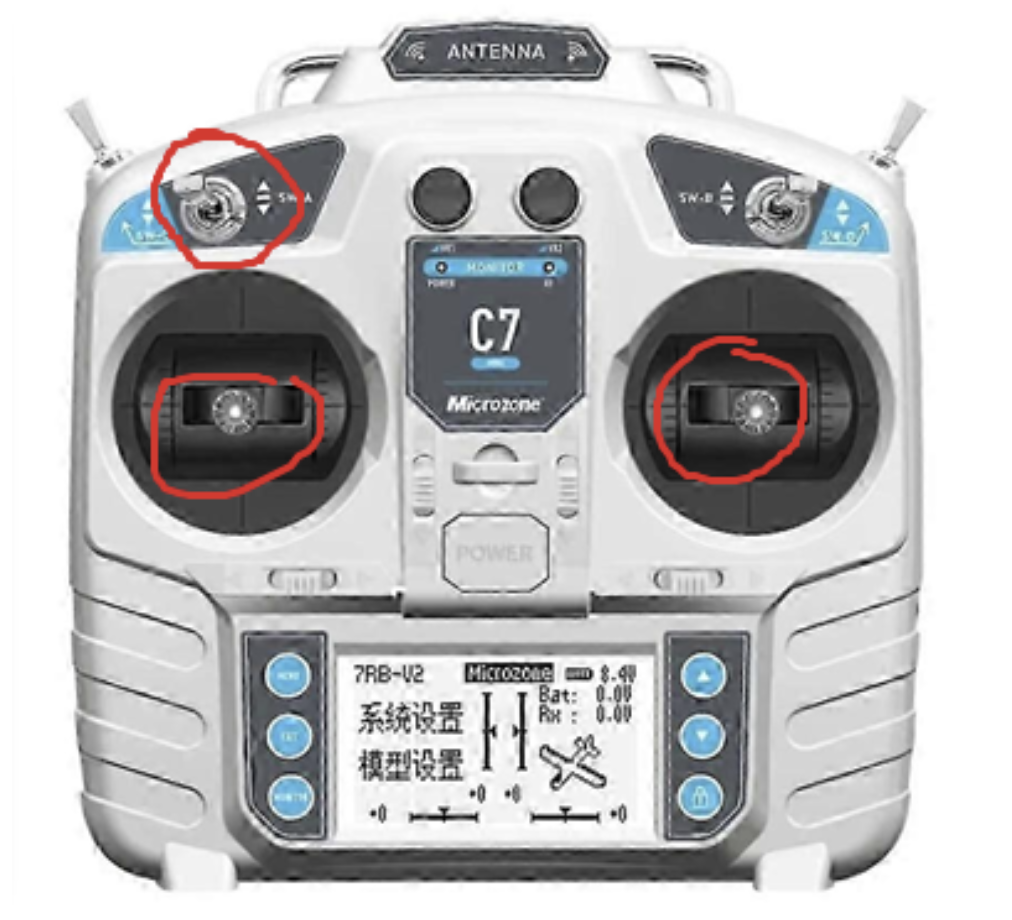
\includegraphics[width=0.72\textwidth]{slike/remote_control.png}
    \caption{Daljinec z ozna\v{c}enimi gumbi in joysticki, ki sem jih testiral in jih uporabljam pri upravljanju kosilnice. Stikalo na vrhu slu\v{z}i za spremembo na\v{c}ina delovanja, joysticka pa za usmerjanje naprej, nazaj, levo in desno.}
    \label{fig:remote-control}
\end{figure}

\begin{figure}[H]
    \centering
    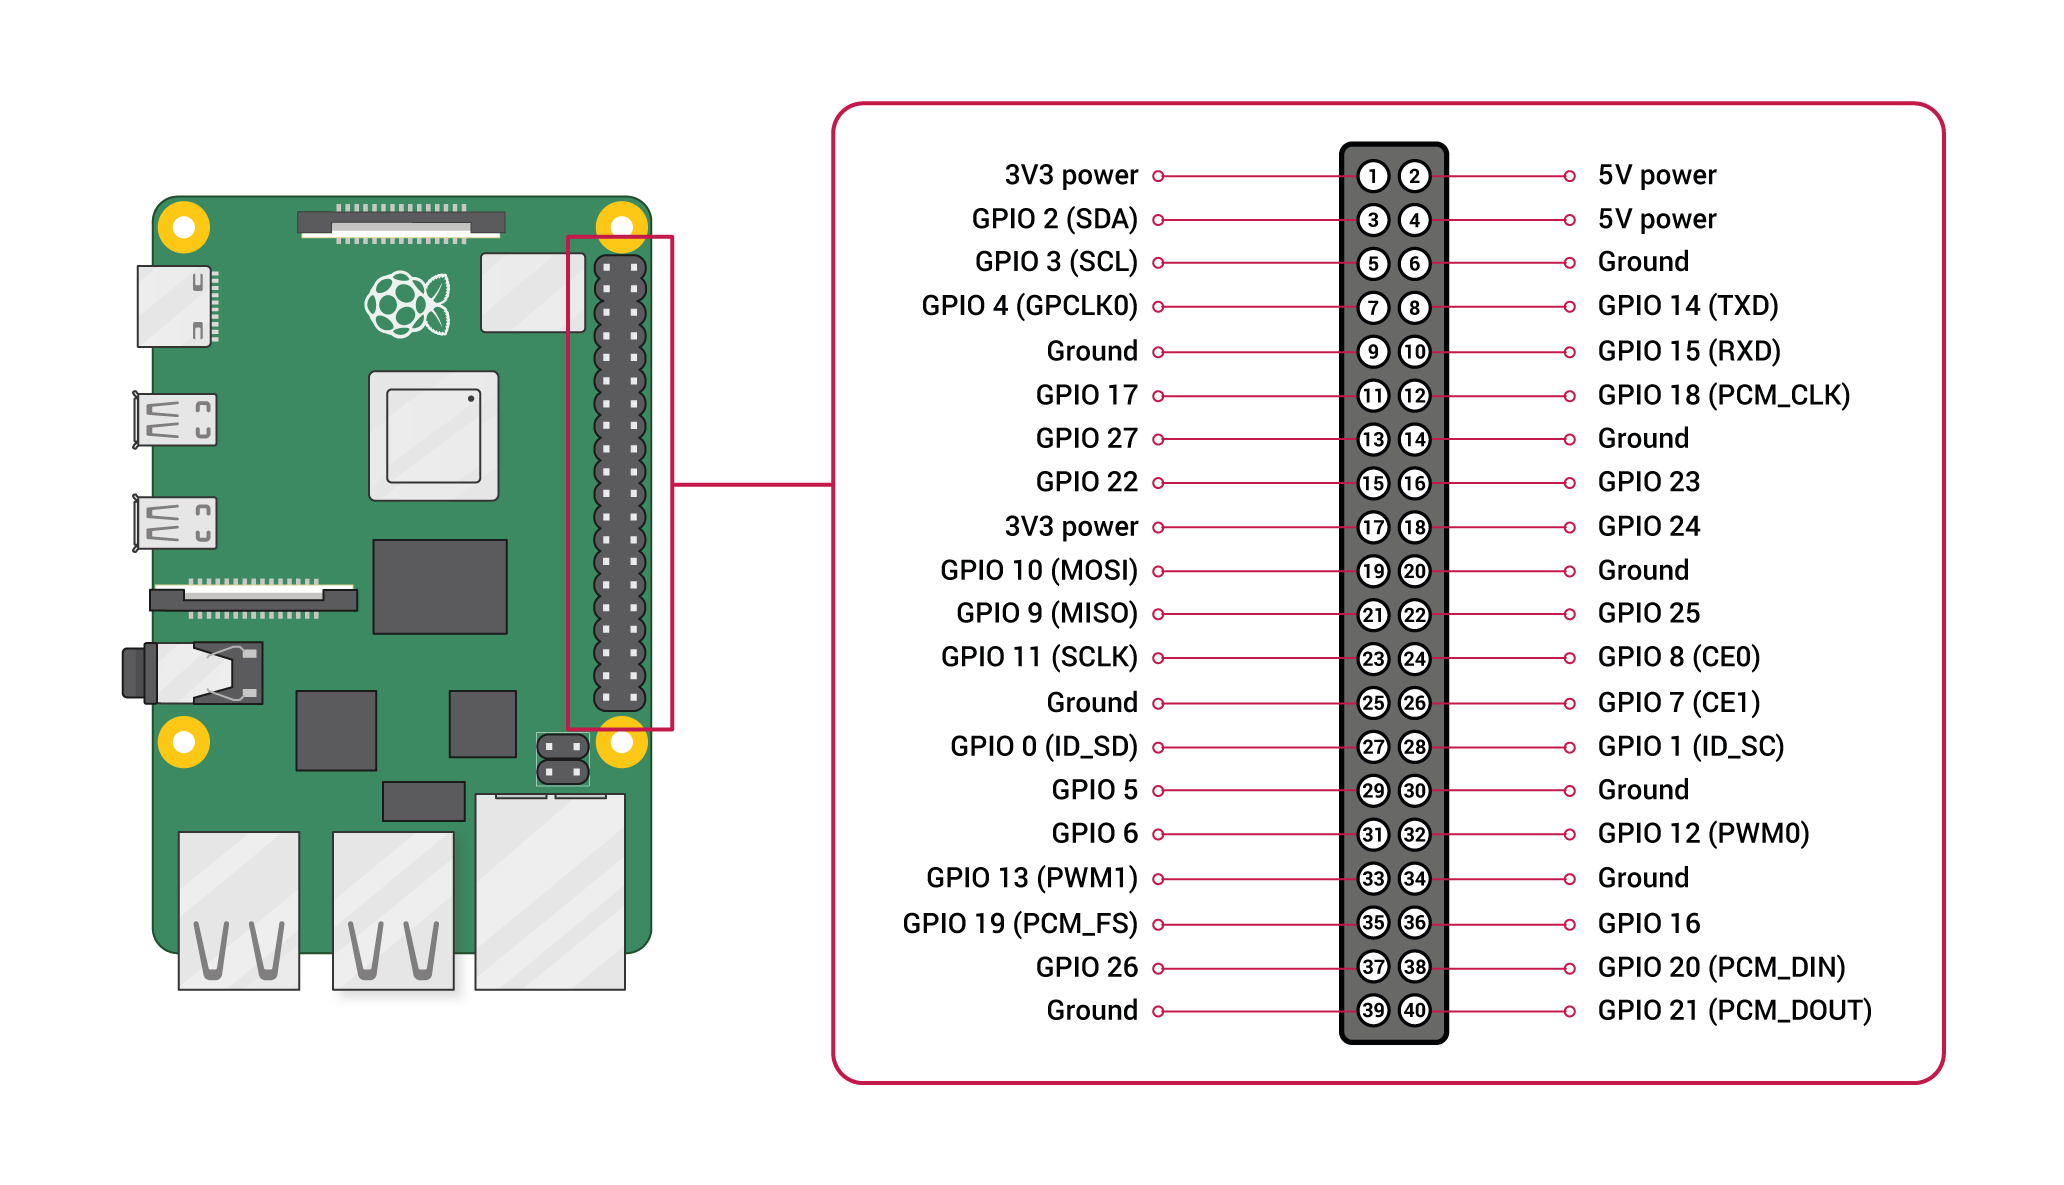
\includegraphics[width=0.72\textwidth]{slike/skica s pojasnsili vseh pinov na raspbery pi.png}
    \caption{Skica Raspberry~Pi z ozna\v{c}enimi pini in navedenim funkcijami PINOV, ki sem jih uporabljal pri povezovanju sistema.}
    \label{fig:rpi-pinout}
\end{figure}

\subsubsection{OpenCV in MobileNetSSD}

OpenCV je odprtokodna knji\v{z}nica za ra\v{c}unalni\v{s}ki vid, ki med drugim vsebuje modul
\texttt{dnn} za poganjanje nevronskih mre\v{z}. Za prepoznavanje objektov sem izbiral med modelom
YOLO, ki je natan\v{c}nej\v{s}i, vendar precej bolj ra\v{c}unsko potraten, in modelom MobileNetSSD, ki je
bil posebej zasnovan za naprave z omejeno procesorsko mo\v{c}jo. Na Raspberry~Pi je bil MobileNetSSD
bistveno hitrej\v{s}i in je dosegal zadovoljivo hitrost prepoznavanja. Nekaj te\v{z}av z natan\v{c}nostjo sem
imel pri testih v temi, vendar se kosilnica v praksi uporablja predvsem podnevi, zato to ni bila
klju\v{c}na omejitev sistema.

\subsubsection{Picamera2}

Picamera2 je uradna Python knji\v{z}nica za upravljanje kamere na Raspberry~Pi. V primerjavi s starej\v{s}o
knji\v{z}nico \texttt{PiCamera} bolje podpira novej\v{s}e kamerne module in se brezhibno integrira z
OpenCV, kar omogo\v{c}a neposreden prenos okvirjev v obliki NumPy matrik brez dodatnih konverzij
\parencite{raspi_camera_software}.

\subsubsection{GNSS modul LC29H z DGPS podporo}

Za natan\v{c}no pozicioniranje sem izbral modul LC29H podjetja Quectel, ki podpira sprejem signalov iz
ve\v{c} satelitskih konstelacij (GPS, GLONASS, Galileo, BeiDou) in sprejem RTCM-diferencialnih
popravkov prek UART-vmesnika. Navadni ceneni GPS-moduli dosegajo natan\v{c}nost pribli\v{z}no
$\pm 5$\,m, moji testi z modulom NEO-7M, ki stane pribli\v{z}no 6\,€, pa so pokazali, da se lahko
natan\v{c}nost v neugodnih razmerah poslab\v{s}a tudi na 30\,m ali ve\v{c}. LC29H z DGPS-popravki dosega
natan\v{c}nost pod 1\,m, kar je klju\v{c}no za smiselno lociranje kosilnice pri delu na daljavo.

\subsubsection{NTRIP in RTK2go}

NTRIP (\textit{Networked Transport of RTCM via Internet Protocol}) je standardiziran protokol za
prenos diferencialnih GPS-popravkov prek interneta v realnem \v{c}asu. Za popravke sem uporabil javno
dostopno storitev RTK2go in referen\v{c}no postajo FRELIH v \v{C}rnem Vrhu nad Idrijo
\parencite{rtk2go}. Testiranja sem izvajal v Cerknem, ki je od postaje oddaljeno pribli\v{z}no 33\,km.
Sicer bi bilo bolje, \v{c}e bi bila referen\v{c}na postaja bli\v{z}je, vendar sem bil med testiranjem
zadovoljen z dose\v{z}eno natan\v{c}nostjo, ki je zna\v{s}ala pribli\v{z}no $\pm 1{,}5$\,m.

\subsubsection{Python in ve\v{c}nitnost}

Celoten sistem sem implementiral v Pythonu~3, ki je standardni jezik za razvoj na Raspberry~Pi.
Posamezne naloge, kot so branje kamere, video stre\v{z}nik, branje GPS, po\v{s}iljanje NTRIP-podatkov
in krmilna zanka, te\v{c}ejo v lo\v{c}enih nitih z modulom \texttt{threading}. Tak pristop omogo\v{c}a, da
sistem ve\v{c} opravil izvaja hkrati, kar je bistveno za dovolj hiter odziv pri delovanju v praksi.

\subsection{Analiza RC-krmiljenja in PWM-meritve}

Ko sem raziskoval daljinski upravljalnik, sem si najprej prebral dokumentacijo sprejemnika MC8RE
\parencite{microzone_mc8re}. Nato sem opravil meritve z Arduino Uno, ki mi je slu\v{z}il kot analogni
merilec pulzov. Napisal sem program, ki je prek analognih pinov meril, s kak\v{s}no frekvenco sprejemnik
oddaja PWM-signal, ki ga prejme od daljinca. Podatke sem prikazal v programu Arduino Serial Plotter
znotraj okolja Arduino~IDE. Tako sem ugotovil, da se posamezna smer prepozna po konkretnih pulznih
\v{s}irinah. Vizualizacija poteka pulzov v realnem \v{c}asu mi je omogo\v{c}ila, da sem la\v{z}je dolo\v{c}il meje
za histerezno logiko.

Pri meritvah sem dobil naslednji vzorec: premik naprej pomeni, da je eden od kanalov pribli\v{z}no
2000\,\textmu{}s, drugi pa pribli\v{z}no 1050\,\textmu{}s. Pri mirovanju sta oba kanala pribli\v{z}no
1500\,\textmu{}s.

\begin{figure}[H]
    \centering
    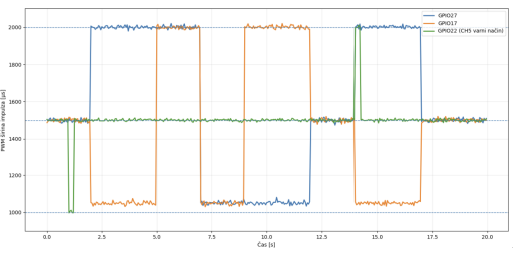
\includegraphics[width=0.85\textwidth]{slike/graf_merjenja_signala.png}
    \caption{Graf meritev PWM-signalov posameznih kanalov, izmerjenih z Arduinom in Serial Plotterjem v Arduino~IDE.}
    \label{fig:graf-kanalov}
\end{figure}

\subsubsection{Varnostna preklopna logika}

Spodnji blok kode prikazuje, kako v glavni zanki preverjam, ali je vrednost kanala CH5, ki je
vezan na stikalo na daljincu, ve\v{c}ja od konstante \texttt{AUTOPILOT\_ON}. V programu sem
nastavil mejo za vklop na 1900\,\textmu{}s, mejo za izklop na 1100\,\textmu{}s, nevtralna
vrednost pa je 1500\,\textmu{}s. \v{C}e se stikalo premakne le za kratek trenutek, se stanje
nastavi na \texttt{True} ali \texttt{False}, nato pa se signal lahko vrne v nevtralno obmo\v{c}je.
Na ta na\v{c}in ostane na\v{c}in delovanja nastavljen glede na zadnji premik stikala.

\begin{lstlisting}[language=Python,caption={Varnostna preklopna logika glede na kanal CH5.}]
if ch5 > AUTOPILOT_ON and not autopilot_mode:
    autopilot_mode = True
elif ch5 < AUTOPILOT_OFF and autopilot_mode:
    autopilot_mode = False
\end{lstlisting}

\subsection{Na\v{c}rt sistema in razvojne iteracije}

\subsubsection{Osnovna arhitektura sistema}

Najprej sem v glavni datoteki definiral osnovno arhitekturo sistema. Uvozil sem vse potrebne
knji\v{z}nice, da sem lahko dosegel \v{z}eleno funkcionalnost. Kot je razvidno iz spodnjega dela kode,
sem uvozil tudi modul \texttt{threading}, saj je bilo zelo pomembno, da sistem hkrati izvaja ve\v{c}
nalog: obdeluje sliko s kamere, oddaja video kot stre\v{z}nik, po potrebi po\v{s}lje signal za
zaustavitev ter sprejema in obdeluje GPS-koordinate skupaj s popravki.

\begin{lstlisting}[language=Python,caption={Osnovna struktura in knji\v{z}nice v final.py.}]
import base64
import json
import socket
import threading
import time
from http.server import HTTPServer, BaseHTTPRequestHandler

import serial
import cv2
from picamera2 import Picamera2
import pigpio
\end{lstlisting}

\subsubsection{Nastavitve za RC, kamero in GNSS}

Tu sem definiral osnovne konstante in preklopne meje na enem mestu, ker sem jih med testiranjem
ve\v{c}krat spreminjal.

V mno\v{z}ici, to je podatkovni strukturi, podobni seznamu, vendar neurejeni, sem definiral imena
objektov, ki jih nevronska mre\v{z}a zazna na sliki. Z dodajanjem drugih imen objektov bi lahko
dosegel, da bi se kosilnica ustavila tudi ob zaznavi drugih predmetov, na primer mobilnega
telefona, vendar to za cilj moje naloge ni bilo potrebno.

\begin{lstlisting}[language=Python,caption={Klju\v{c}ne nastavitve za signalne pragove in zaznavo.}]
CH1_IN = 17;  CH2_IN = 27;  CH5_IN = 22
CH1_OUT = 23; CH2_OUT = 24

MIN_PULSE = 900;  MAX_PULSE = 2100;  NEUTRAL_PULSE = 1500
AUTOPILOT_ON = 1900;  AUTOPILOT_OFF = 1100
CONF_THRESH = 0.5
TARGETS = {"person", "cat", "dog"}
\end{lstlisting}

\subsubsection{Glavna zanka programa}

Glavna zanka programa povezuje vse podsisteme v enoten sistem. V funkciji \texttt{main()} se
najprej odpre serijska povezava z GNSS-modulom, nato pa se za posamezne naloge za\v{z}enejo lo\v{c}ene
niti. Ena nit skrbi za branje GNSS-podatkov, druga za povezavo z NTRIP-stre\v{z}nikom, tretja za
zajem slike s kamere, \v{c}etrta za video tok, dodatna nit pa za spletni stre\v{z}nik uporabni\v{s}kega
vmesnika. Na koncu se za\v{z}ene \texttt{control\_loop()}, ki neprekinjeno izvaja glavno krmilno logiko.

\begin{lstlisting}[language=Python,caption={Glavna funkcija programa in zagon vseh niti.}]
def main():
    ser = serial.Serial(SERIAL_PORT, SERIAL_BAUD, timeout=1)
    print("[INFO] GNSS serial open:", SERIAL_PORT, SERIAL_BAUD)

    threading.Thread(target=gnss_reader_thread, args=(ser,), daemon=True).start()
    threading.Thread(target=ntrip_manager_thread, args=(ser,), daemon=True).start()
    threading.Thread(target=camera_thread, daemon=True).start()
    threading.Thread(target=mjpeg_stream_thread, daemon=True).start()

    threading.Thread(
        target=lambda: HTTPServer(("0.0.0.0", HTTP_PORT), DashboardHandler).serve_forever(),
        daemon=True
    ).start()

    control_loop()
\end{lstlisting}

Tak\v{s}na zasnova omogo\v{c}a, da sistem ve\v{c} funkcij izvaja hkrati in da posamezen podsistem ne
blokira delovanja drugih.

\subsubsection{Stre\v{z}nik in uporabni\v{s}ki vmesnik}

Pomemben del sistema je bil tudi spletni stre\v{z}nik, ki operaterju omogo\v{c}a dostop do slike s
kamere in do trenutnega polo\v{z}aja kosilnice. Stre\v{z}nik je pripravljen tako, da ob obisku osnovnega
naslova vrne HTML-stran z uporabni\v{s}kim vmesnikom, ob zahtevi na naslov \texttt{/pos} pa vrne
trenutne GPS-podatke v obliki JSON. Na ta na\v{c}in lahko brskalnik sproti osve\v{z}uje polo\v{z}aj
kosilnice in ga prikazuje na zemljevidu.

\begin{lstlisting}[language=Python,caption={Osnovni del stre\v{z}nika za po\v{s}iljanje HTML-strani in GPS-podatkov.}]
class DashboardHandler(BaseHTTPRequestHandler):
    def do_GET(self):
        if self.path == "/" or self.path == "/index.html":
            self.send_response(200)
            self.send_header("Content-Type", "text/html; charset=utf-8")
            self.end_headers()
            self.wfile.write(INDEX_HTML)
            return

        if self.path == "/pos":
            with state_lock:
                data = json.dumps(latest).encode("utf-8")
            self.send_response(200)
            self.send_header("Content-Type", "application/json; charset=utf-8")
            self.end_headers()
            self.wfile.write(data)
            return
\end{lstlisting}

Na strani odjemalca sem uporabil JavaScript, ki v rednih \v{c}asovnih presledkih po\v{s}ilja zahteve na
\texttt{/pos} in posodablja podatke na zemljevidu. Hkrati se nalo\v{z}i tudi video tok z naslova
\texttt{/stream}, zato lahko operater na enem mestu spremlja sliko in lokacijo.

\begin{lstlisting}[language=JavaScript,caption={Periodi\v{c}no pridobivanje polo\v{z}aja in posodabljanje zemljevida.}]
async function pollPos(){
  try{
    const r = await fetch('/pos', { cache:'no-store' });
    if(!r.ok) throw new Error('HTTP ' + r.status);
    const d = await r.json();

    if(d.lat == null || d.lon == null){
      posPill.textContent = '/pos: no data';
      return;
    }

    marker.setLatLng([d.lat, d.lon]);
  }catch(e){
    posPill.textContent = '/pos: ERROR';
  }
}

setInterval(pollPos, 500);
\end{lstlisting}

Tak\v{s}na zasnova stre\v{z}nika je bila zame primerna predvsem zato, ker je preprosta, pregledna in
dovolj hitra za delovanje na Raspberry~Pi.

Pomembno mi je bilo tudi, da so funkcije napisane tako, da sem lahko vsak podsistem testiral
posebej. Tako sem najprej lo\v{c}eno preveril delovanje kamere, GPS-a, NTRIP-povezave, spletnega
vmesnika in RC-krmiljenja, \v{s}ele nato pa sem vse dele zdru\v{z}il v kon\v{c}no datoteko
\texttt{final.py}.

\subsection{Varnostni mehanizem samodejne zaustavitve}

Pri varnostnem podsistemu sem najprej naredil osnovno razli\v{c}ico, ki je kosilnico ustavila takoj,
ko je kamera zaznala \v{c}loveka, psa ali ma\v{c}ko. Opazil sem, da je imel sistem v\v{c}asih te\v{z}avo, da je
oviro zaznal le v enem okvirju, zato se kosilnica ni vedno ustavila dovolj zanesljivo. Zato sem
dodal \v{c}asovni zamik, kar pomeni, da kosilnica po zaznavi ovire obstane \v{s}e eno sekundo in \v{s}ele
nato ponovno preveri, ali je objekt \v{s}e vedno pred njo. \v{C}e objekt ni ve\v{c} prisoten, sistem nadaljuje
delovanje.

\subsubsection{Sprotna zaustavitev ob zaznavi \v{c}loveka}

Ko je varnostni re\v{z}im vklju\v{c}en, sem moral zagotoviti, da motorja takoj dobita nevtralni pulz.
Ker program deluje v ve\v{c} nitih hkrati, sem \v{z}elel, da se kosilnica ustavi ne glede na trenutno
obremenitev drugih delov sistema. Zato sem v glavni krmilni zanki ob zaznavi cilja ali ob aktivnem
varnostnem zadr\v{z}anju obema izhodoma takoj nastavil nevtralno vrednost. Tako sem dosegel hiter in
zanesljiv odziv.

\begin{lstlisting}[language=Python,caption={Samodejna zaustavitev ob zaznanih preprekah.}]
if autopilot_mode and (target_detected or safety_latched):
    pi.set_servo_pulsewidth(CH1_OUT, NEUTRAL_PULSE)
    pi.set_servo_pulsewidth(CH2_OUT, NEUTRAL_PULSE)
else:
    pi.set_servo_pulsewidth(CH1_OUT, ch1)
    pi.set_servo_pulsewidth(CH2_OUT, ch2)
\end{lstlisting}

\subsubsection{Clear-delay logika}

V tem delu je opisan sistem odlo\v{c}anja, ali varnostni mehanizem ostane aktiven ali ne. Program v
spremenljivko zapi\v{s}e \v{c}as, ko je bila ovira nazadnje zaznana, nato pa preverja, ali je od tega
trenutka pretekla vsaj ena sekunda. \v{C}e ovire v tem \v{c}asu ni ve\v{c}, se varnostni mehanizem sprosti
in program nadaljuje normalno delovanje. S tem sem prepre\v{c}il, da bi se sistem ob kratkotrajni
prekinitvi zaznave prehitro ponovno zagnal.

\begin{lstlisting}[language=Python,caption={1-sekundni zamik pri ponovni sprostitvi varnostne zaustavitve.}]
if target_detected:
    safety_latched = True
    target_clear_since = None
else:
    if safety_latched:
        if target_clear_since is None:
            target_clear_since = now
        elif (now - target_clear_since) >= CLEAR_DELAY_S:
            safety_latched = False
            target_clear_since = None
\end{lstlisting}

\subsubsection{Zaznava objektov s MobileNetSSD}

Uporabil sem MobileNetSSD, ker sem ugotovil, da je za Raspberry~Pi pomembnej\v{s}a hitrost kot
maksimalna natan\v{c}nost. YOLO sem preizkusil, vendar je bil za moj sistem prepo\v{c}asen, saj je
prepoznava trajala pribli\v{z}no dve sekundi, kar bi v praksi pomenilo prepozen odziv. Sliko pri
prepoznavi zmanj\v{s}am na 160 $\times$ 160 pikslov, saj je tako obdelava hitrej\v{s}a. Glede na teste se
natan\v{c}nost zaradi tega ni toliko zmanj\v{s}ala, da bi sistem postal neuporaben. Pri tak\v{s}nih sistemih
je treba poiskati primerno razmerje med natan\v{c}nostjo in hitrostjo obdelave slike.

\begin{lstlisting}[language=Python,caption={Zaznavanje tar\v{c}.}]
small = cv2.resize(current_frame, (160, 160))
blob = cv2.dnn.blobFromImage(small, 0.007843, (160, 160), 127.5)

net.setInput(blob)
detections = net.forward()

detected_now = any(
    float(detections[0, 0, i, 2]) >= CONF_THRESH and
    CLASSES[int(detections[0, 0, i, 1])] in TARGETS
    for i in range(detections.shape[2])
)
\end{lstlisting}

\subsubsection{Zmanj\v{s}anje zakasnitve video toka}

Video tok sem namensko stisnil in zmanj\v{s}al kakovost slike, ker sem ugotovil, da je za varnostni
prikaz pomembnej\v{s}a odzivnost kot popolna ostrina vsakega okvirja. Sprva se je slika posodabljala
pribli\v{z}no vsakih 1{,}5\,s, zato sem zmanj\v{s}al lo\v{c}ljivost in omogo\v{c}il kompresijo, da se je video
na stre\v{z}niku, do katerega sem dostopal prek telefona, posodabljal s pribli\v{z}no 0{,}5\,s zamika.
To je bilo dovolj hitro za varno vo\v{z}njo na daljavo.

\begin{lstlisting}[language=Python,caption={MJPEG-stre\v{z}nik z zmerno kakovostjo JPEG.}]
ok, jpeg = cv2.imencode('.jpg', current_frame,
                         [cv2.IMWRITE_JPEG_QUALITY, 45])
if ok:
    self.wfile.write(b'--frame\r\n')
    self.wfile.write(b'Content-Type: image/jpeg\r\n\r\n')
    self.wfile.write(jpeg.tobytes())
    self.wfile.write(b'\r\n')
\end{lstlisting}

\subsection{GNSS, DGPS in NTRIP v praksi}

\subsubsection{Delovanje GPS in omejitve navadnih modulov}

GPS deluje na podlagi izmere \v{c}asa, ki ga signal potrebuje, da potuje od satelita do sprejemnika.
Ker signal potuje s svetlobno hitrostjo, sprejemnik iz razlik v \v{c}asih sprejema od vsaj \v{s}tirih
satelitov izra\v{c}una svoj prostorski polo\v{z}aj. Natan\v{c}nost je odvisna od geometrije satelitov,
atmosferskih pojavov, odbojev signalov in kakovosti sprejemnika. Evropska vesoljska agencija v
svojih navodilih za satelitsko navigacijo poudarja, da je za vi\v{s}jo natan\v{c}nost potrebna dodatna
korekcijska plast \parencite{esa_satnav}.

Navadni ceneni GPS-moduli dosegajo natan\v{c}nost okrog $\pm 5$\,m, ki pa se lahko nenadoma
poslab\v{s}a na 30\,m ali ve\v{c}, kadar imamo omejen pogled na nebo ali ko signal odbijajo okoli\v{s}ki
predmeti. Za kosilnico, ki jo operater vodi na daljavo in je morda ne vidi neposredno, je tak\v{s}na
nenatan\v{c}nost polo\v{z}aja nezanesljiva in potencialno nevarna. Zato sem moral poiskati natan\v{c}nej\v{s}o
re\v{s}itev.

\subsubsection{Diferencialni GPS in NTRIP}

Diferencialni GPS (DGPS) deluje tako, da referen\v{c}na postaja na znani lokaciji neprestano meri
napako GPS-a in te popravke v obliki RTCM-sporo\v{c}il po\v{s}ilja sprejemniku v terenu. Sprejemnik nato
od\v{s}teje izmerjeno napako in dobi bistveno bolj stabilen polo\v{z}aj. Uradna dokumentacija u-blox
opisuje GNSS kot skupino sistemov za dolo\v{c}anje polo\v{z}aja z ve\v{c} satelitskimi konstelacijami
\parencite{ublox_gnss}.

V mojem projektu sem za popravke uporabil javno dostopno storitev RTK2go in referen\v{c}no postajo
FRELIH v \v{C}rnem Vrhu nad Idrijo \parencite{rtk2go}. Testiranja sem izvajal v Cerknem, ki je od
postaje oddaljeno okrog 33\,km, kar je bilo za moje potrebe \v{s}e uporabno.

\begin{figure}[H]
    \centering
    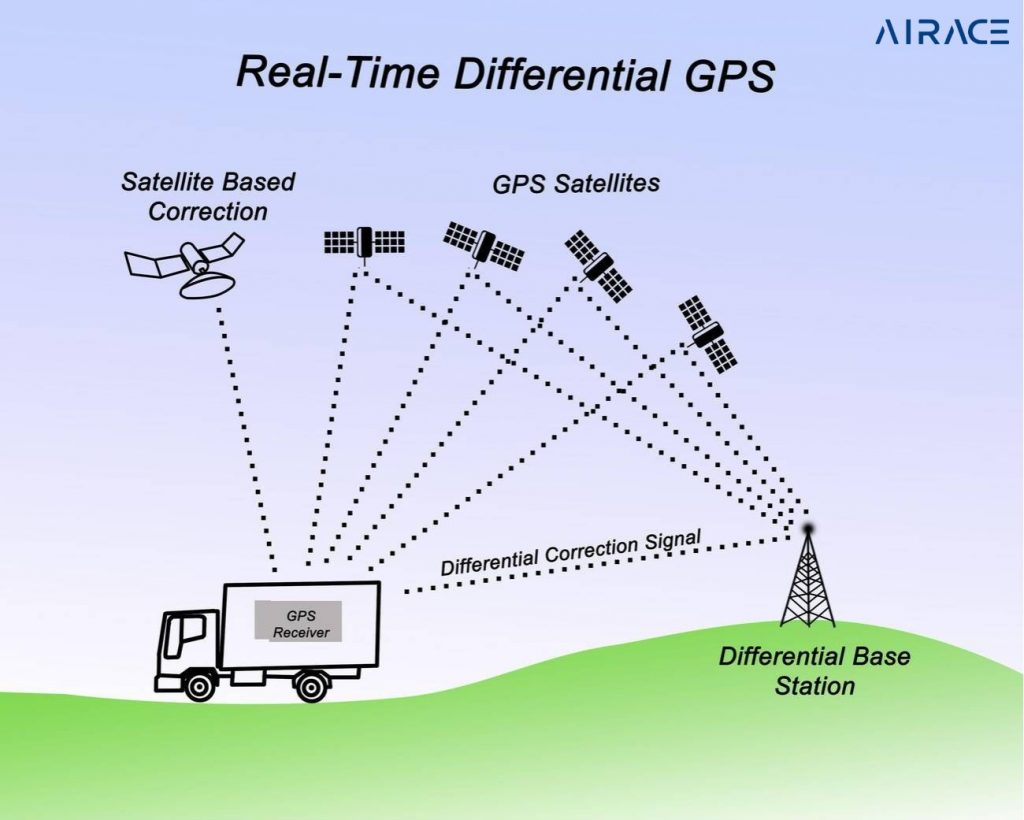
\includegraphics[width=0.80\textwidth]{slike/DGPS SKETCH.jpg}
    \caption{Prikaz principa delovanja diferencialnega GPS in popravkov NTRIP \parencite{airace_dgps}.}
    \label{fig:dgps-sketch}
\end{figure}

\subsubsection{Povezava na NTRIP in po\v{s}iljanje GGA}

Sprejemnik prek serijskega vmesnika po\v{s}ilja NMEA-stavke, med katerimi je klju\v{c}en GGA
(\textit{Global Positioning System Fix Data}). Tega po\v{s}iljamo nazaj na NTRIP-caster, ki v zameno
vrne RTCM-korekcijske podatke.

Za tak\v{s}no delovanje je potrebna stalna povezava z internetom. Zato sem sistem med testiranjem
povezal na dostopno to\v{c}ko mobilnega telefona, ki je bil povezan v mobilno omre\v{z}je. Druga mo\v{z}nost
bi bila uporaba lo\v{c}enega mobilnega Wi-Fi-modema, ki bi omogo\v{c}al enako funkcionalnost tudi brez
telefona.

\begin{lstlisting}[language=Python,caption={Vzpostavitev povezave na NTRIP-caster in po\v{s}iljanje GGA-stavka.}]
sock = socket.create_connection((NTRIP_HOST, NTRIP_PORT),
                                 timeout=10)
auth = base64.b64encode(
    f"{USERNAME}:{PASSWORD}".encode()).decode()
req = (
    f"GET /{MOUNTPOINT} HTTP/1.0\r\n"
    f"User-Agent: Python-NTRIP\r\n"
    f"Authorization: Basic {auth}\r\n\r\n"
)
sock.sendall(req.encode("ascii", errors="ignore"))
\end{lstlisting}

V praksi sem ugotovil, da se natan\v{c}nost z DGPS-popravki izbolj\v{s}a dovolj, da je polo\v{z}aj dejansko
uporaben za orientacijo pri daljinskem delu.

\subsection{Spletni vmesnik za operaterja}

Spletni vmesnik sem izdelal zato, da sem lahko sistem spremljal brez neposrednega priklopa z
kablom na Raspberry~Pi in brez branja surovih podatkov prek terminala. Povezava prek omre\v{z}ja Wi-Fi
je to bistveno poenostavila. Kosilnica v \v{z}ivo pretaka video s kamere in po\v{s}ilja svoj polo\v{z}aj,
ki se nato prika\v{z}e na odprtokodnem zemljevidu Leaflet. Vmesnik sem razvil v HTML-ju in
JavaScriptu brez dodatnih stre\v{z}ni\v{s}kih ogrodij, ker sem \v{z}elel, da sistem ostane \v{c}im bolj
preprost za vzdr\v{z}evanje.

Ugotovil sem, da sta video slika in prikaz polo\v{z}aja skupaj veliko bolj uporabna kot zgolj surovi
podatki. Operater lahko takoj vidi, ali je sistem na pravem mestu in ali je kosilnica pravilno
usmerjena.

\begin{figure}[H]
    \centering
    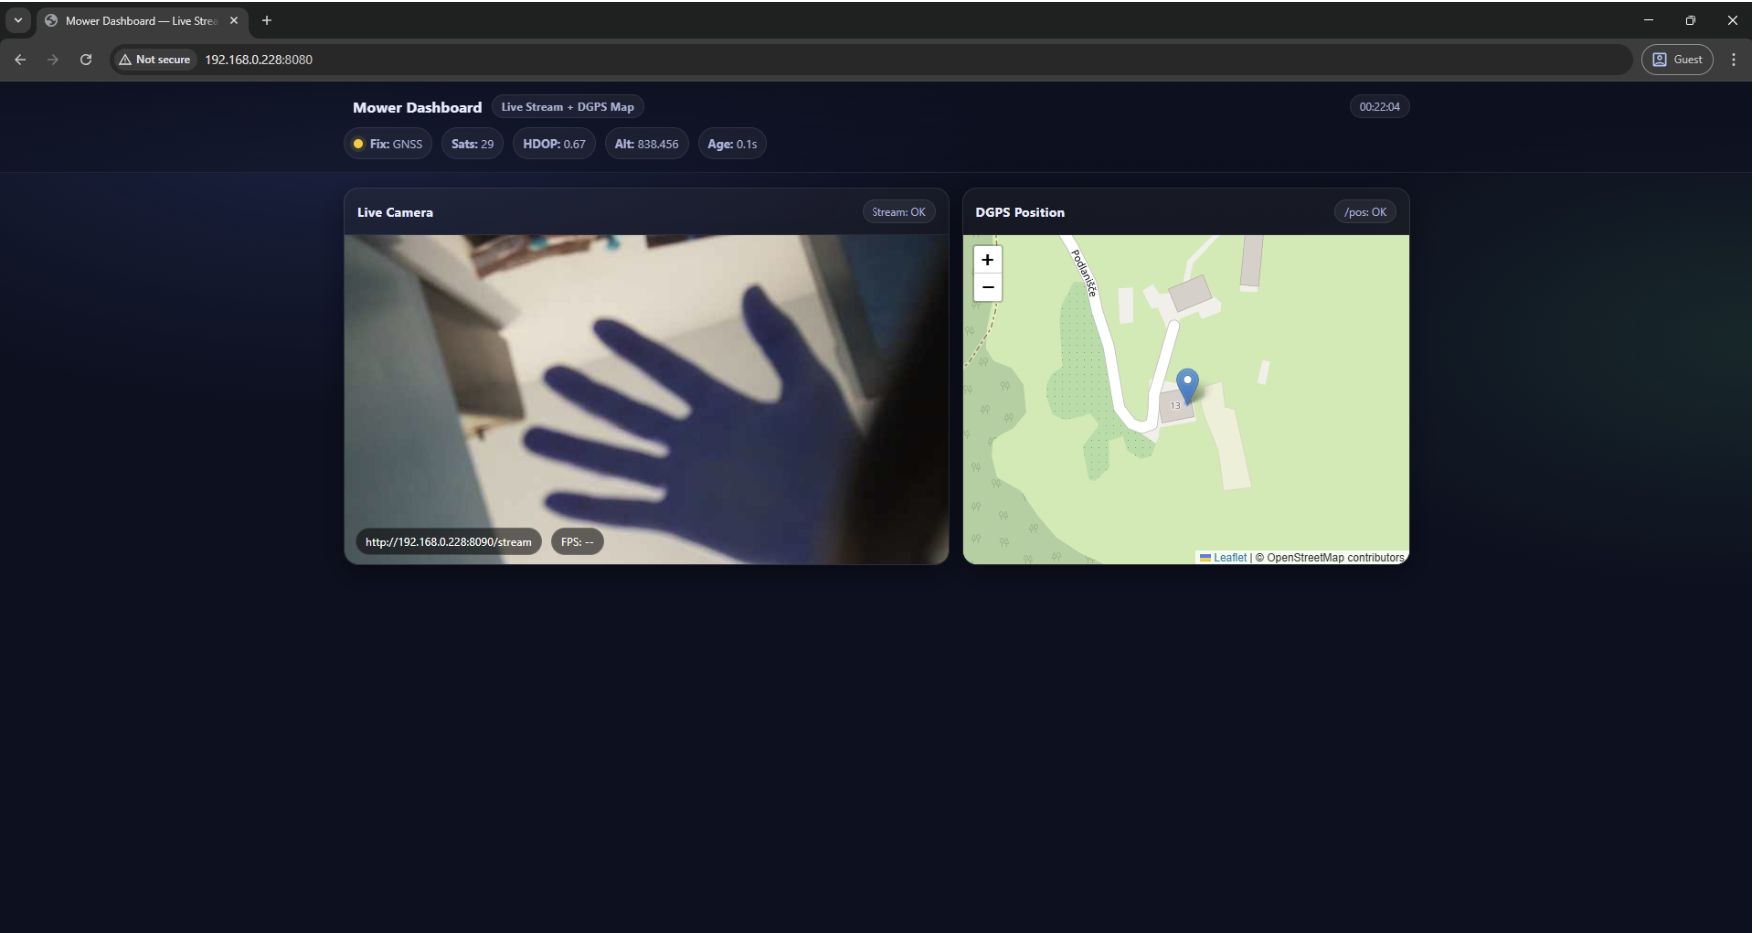
\includegraphics[width=0.84\textwidth]{slike/web_interface.png}
    \caption{Spletni vmesnik z \v{z}ivim videoposnetkom kamere in GPS-lokacijo kosilnice na interaktivnem zemljevidu.}
    \label{fig:web-interface}
\end{figure}

\subsection{Testiranje sistema in analiza rezultatov}

Preden sem zdru\v{z}il vse v kon\v{c}no skripto, sem moral posamezne dele preizkusiti lo\v{c}eno. Zato sem
uporabil skripto za kamero, prikaz PWM-signalov ter lo\v{c}en preizkus NTRIP-povezave. To mi je
pomagalo, da sem odkril te\v{z}ave, preden so postale del ve\v{c}je skripte.

Ena od napak, ki sem jo na\v{s}el, je bila, da se je kamera pri preveliki lo\v{c}ljivosti prepo\v{c}asi
odzivala. Zato sem zmanj\v{s}al velikost vhodne slike in inferenco izvajal samo na vsakem drugem
okviru. Druga te\v{z}ava je bila, da sem moral zelo natan\v{c}no dolo\v{c}iti prage za CH5, ker se je sicer
na\v{c}in delovanja nepredvidljivo spreminjal med varnostnim in obi\v{c}ajnim re\v{z}imom. Pri GPS-delu pa
sem ugotovil, da brez RTK-popravkov polo\v{z}aj preve\v{c} niha, zato sem uporabil NTRIP-povezavo za
natan\v{c}nej\v{s}o lokacijo.

Med terenskim testiranjem sem preveril odzivni \v{c}as od zaznave do ustavitve ter stabilnost
GPS-polo\v{z}aja. Sistem je zaustavil kosilnico v manj kot 100\,ms od zaznave osebe pri razdalji do
4\,m in zadostnih svetlobnih razmerah. GPS-natan\v{c}nost je bila z DGPS-popravki stabilna pod 1\,m,
v primerjavi s $\pm 5$\,m ali ve\v{c} brez popravkov.

\begin{figure}[H]
    \centering
    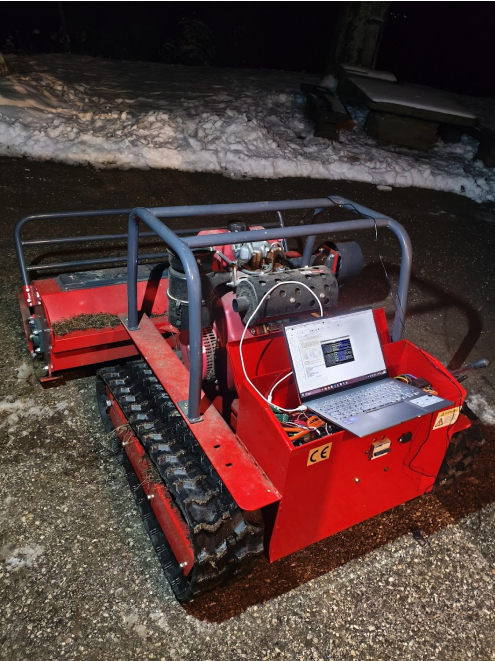
\includegraphics[width=0.82\textwidth]{slike/testiranje_na_terenu.png}
    \caption{Testiranje sistema na terenu: mul\v{c}er od dale\v{c} s prenosnim ra\v{c}unalnikom med preizkusi.}
    \label{fig:testiranje-teren}
\end{figure}

\begin{figure}[H]
    \centering
    \includegraphics[width=0.78\textwidth]{slike/slika_notranjosti_mulcerja.png}
    \caption{Notranjost mul\v{c}erja z dodanim Raspberry~Pi ra\v{c}unalnikom in name\v{s}\v{c}eno elektroniko.}
    \label{fig:mulcer-inside}
\end{figure}

\begin{figure}[H]
    \centering
    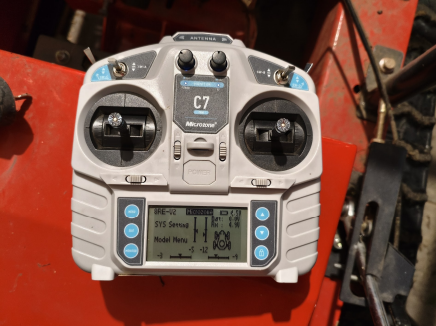
\includegraphics[width=0.72\textwidth]{slike/daljinec_na_mulcerju.png}
    \caption{Daljinec, name\v{s}\v{c}en na mul\v{c}erju med terenskim testiranjem.}
    \label{fig:daljinec-na-mulcerju}
\end{figure}

% ==============================================================
%  3  ZAKLJUCEK
% ==============================================================
\section{Zaklju\v{c}ek}

V seminarski nalogi sem predstavil nadgradnjo daljinsko vodene kosilnice z ra\v{c}unalni\v{s}kim vidom,
spletnim vmesnikom in natan\v{c}nej\v{s}im dolo\v{c}anjem polo\v{z}aja. Projekt sem zasnoval od izbire
strojne opreme in programske arhitekture do implementacije glavnih funkcionalnosti, kot so
zaznavanje ljudi in \v{z}ivali, samodejna zaustavitev, prenos video slike in prikaz lokacije na
zemljevidu.

Pri delu sem ugotovil, da so si posamezni deli sistema na prvi pogled videti razmeroma preprosti,
v praksi pa se pri vsakem pojavijo nove te\v{z}ave. Posebej pomembno je bilo uskladiti hitrost
zaznavanja, zakasnitev video prenosa in zanesljivost varnostne logike. Pokazalo se je, da pri
tak\v{s}nem sistemu ni najpomembnej\v{s}a samo teoreti\v{c}na natan\v{c}nost, temve\v{c} predvsem dovolj hiter in
zanesljiv odziv v resni\v{c}nem okolju.

Skozi razvoj projekta sem pridobil veliko prakti\v{c}nih izku\v{s}enj s podro\v{c}ja ra\v{c}unalni\v{s}kega vida,
ve\v{c}nitnega programiranja, GNSS-lociranja, spletnih vmesnikov in povezovanja elektronskih modulov
v enoten sistem. Pomembno je bilo tudi to, da sem posamezne podsisteme najprej testiral lo\v{c}eno in
jih \v{s}ele nato zdru\v{z}il v kon\v{c}ni program \texttt{final.py}.

Rezultati ka\v{z}ejo, da sem zastavljeni cilj v veliki meri dosegel. Sistem zna zaznati nevarno bli\v{z}ino
\v{c}loveka ali \v{z}ivali in kosilnico pravo\v{c}asno ustaviti, poleg tega pa operaterju omogo\v{c}a spremljanje
slike in polo\v{z}aja na daljavo. Kljub temu ostajajo mo\v{z}nosti za nadaljnjo nadgradnjo. Za ve\v{c}jo
natan\v{c}nost zaznavanja bi lahko uporabil novej\v{s}i modul Raspberry~Pi Camera AI, ki ima namensko
strojno podporo za obdelavo slike \v{z}e na samem kamerinem modulu, ali zmogljivej\v{s}i ra\v{c}unalnik.
Sistem bi bilo mogo\v{c}e izbolj\v{s}ati tudi z dodatno osvetlitvijo za delo v slab\v{s}ih svetlobnih
razmerah ter z nadaljnjo optimizacijo zakasnitev.

Projekt mi predstavlja trdno osnovo za nadaljnji razvoj in nadgrajevanje, hkrati pa sem z njim
pokazal, da je mogo\v{c}e tudi z razmeroma dostopno opremo izdelati uporaben in varnostno smiseln
sistem za podporo pri daljinskem upravljanju delovnega stroja.

% ==============================================================
%  PRILOGE
% ==============================================================
\appendix
\section{Dodatni viri in demonstracija}

\subsection{Video demonstracija sistema}
Video demonstracija delovanja avtopilota z ra\v{c}unalni\v{s}kim vidom in GPS-lociranjem je dostopna na naslednjem naslovu:
\url{https://drive.google.com/file/d/1oJzYue71dO5h15cRMGLaXBiq_ljRqebY/view?usp=sharing}

Video prikazuje delovanje sistema v realnih pogojih, vklju\v{c}eno zaznavanje ljudi in \v{z}ivali ter odziv varnostnega mehanizma.

% ==============================================================
%  4  VIRI IN LITERATURA
% ==============================================================
\newpage
\printbibliography[heading=bibintoc, title={Viri in literatura}]

% ==============================================================
%  IZJAVA O AVTORSTVU
% ==============================================================
\newpage
\begin{samepage}
\thispagestyle{empty}
\section*{Izjava o avtorstvu}
Izjavljam, da je seminarska naloga v celoti moje avtorsko delo, ki sem ga izdelal samostojno s
pomo\v{c}jo navedene literature in pod vodstvom mentorja.

\vfill

\today \hfill Lin \v{C}ade\v{z}

\vspace{3cm}
\end{samepage}

\end{document}